\section{System Architecture}
\label{sec:system_architecture}

A \projectname{} \emph{cluster} can contain multiple \emph{nodes}, each with a unique id. All the nodes in the cluster store the same number of \emph{stores} - which correspond to database tables. General usage patterns have shown that a site-facing feature may map to either one store or multiple stores. For example, a feature dealing with group recommendation will map to two stores: one recording member id to recommended group ids and second recording a group id to their corresponding description. Every store has the following list of configurable parameters, which are identical to Dynamo's parameters. 
\begin{itemize}
	\item \emph {Replication factor} ($N$) - Number of nodes onto which each key-value tuple is replicated
	\item \emph {Required reads} ($R$) - Number of nodes which we read from in parallel during a $get$ before declaring a success
	\item \emph {Required writes} ($W$) - Number of node responses we block for before declaring success during a $put$
	\item \emph {Key/Value serializer and compression} - \projectname{} can have different serialization schema for key and value. For our custom batch data we use our own custom binary JSON format. \projectname{} also supports per-tuple based compression that can be applied to either key, or value, or both. The serialization / compression is completely dealt by a component which resides on the client side with the server only dealing with raw byte arrays. The only exception to this is a relatively new feature called `server side transforms', which will be further discussed later. 
	\item \emph {Storage type} - \projectname{} supports various read-write storage engine formats: Berkeley DB Java Edition, in-memory hash map and MySQL. We also support our own custom read-only storage engine, which is the focus of this paper.  
\end{itemize}

\begin{figure}
  \centering
    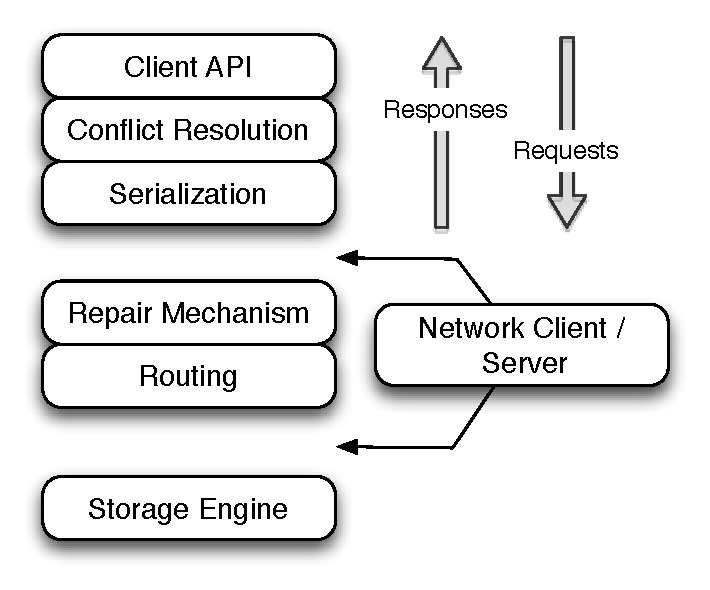
\includegraphics[scale=0.45]{images/arch.pdf}
  \caption{\projectname{} architecture stack}
  \label{arch}
\end{figure}

\projectname{} has a pluggable architecture as shown in Figure \ref{arch}. Each box represents a module, all of which share the same code interface. Every module has exactly one functionality, which we'll explain in the following sub-sections, making it easy to interchange modules and place them in any order. For example, we can have the routing module on either the client side or the server side. Functional separation at the module level also allows us to easily mock these modules for testing purposes. One of the most common use of this can be found in our unit tests where we mock the storage layer to use an in-memory hash map based engine for quick results.  

Most of our modules have been motivated from the original Dynamo paper. But since \projectname{}, like Dynamo, was initially built only for read-write operations we also explain how we had to modify these modules for the batch scenario. Starting from the top our client has a simple $get$ and $put$ API as shown in Figure \ref{clients}. We do not support complex operations like joins, foreign key constraints, etc. The $put$ operations throw an error for the read-only storage engine since we only support bulk loads into them. 

\begin{figure}
\scriptsize
\begin{verbatim}
VectorClock<V> get (K key)
put (K key, VectorClock<V> value)
VectorClock<V> get (K key, T transform)
put (K key, VectorClock<V> value, T transform)
\end{verbatim}
\normalsize

\caption{Operations supported by clients}
  \label{clients}
\end{figure}

During a $put$ to one of the read-write storage engines, we update some replicas of a key asynchronously and allow some failures. Due to common network partitions, we need the ability to version every tuple so as to resolve any conflicts later during $get$s. For the same we use the concept of vector clocks \cite{lamport} as described in the Dynamo paper. In the read-only scenario we do not need the vector clocks since the only way to update data is by bulk loading. Further since our bulk loading operation is atomic we thereby update all the replicas of a key at once. The next two functions show a very powerful feature in \projectname{} which allows you to run a transform / function on your data when it is on the server side. This can help us in saving some network bandwidth by transferring only the required parts of a large value. A common example of this is when we have a list of entities as the value. We can then run a transformed $get$ to retrieve a sub-list or a transformed $put$ to append an entity to your list. 

The next module in the architecture deals with conflict resolution for read-write stores. This module deals with the various conflicting versions of a tuple and finally returns one version. This module can easily be extended by the user to write custom application specific resolution logic. This resolution problem does not apply for read-only stores since the replicas of a key in these stores are always in sync. Similarly the `repair mechanism' layer is used only by the read-write stores to bring the data back to a consistent state. \projectname{} provides two consistency mechanisms: read repair and hinted handoff. Read repair picks the versioned tuple from the conflict resolution module during read-time and updates the inconsistent replicas asynchronously. The other consistency mechanism, hinted handoff, is triggered during write time. If during a $put$ we find that some of the destination nodes are down (and we have satisfied $W$ replicas) the client triggers an asynchronous write to a special store called `slop store' on one of the live nodes. We write a `hint' to this store - where a hint contains the node id of the down node along with the updated value that it missed. We then have a periodic background job running on every node which tries to push these `hints' out to the down nodes.

Since \projectname{} can be thought of as a massive hash table we need a way to partition the data across the multiple servers. The `routing' module deals with partitioning as well as replication. Our partitioning scheme is similar to Dynamo's `virtual nodes' along with consistent hashing approach. We split our hash ring into equal size `partitions' and then assign these partitions to nodes. We share this ring with all the stores, which means changes in the ring require us to change all the stores. Now to generate the `preference list' (list of node ids where the replicas will be stored), we first hash the key to a range belonging to a partition and then continue jumping the ring clockwise till we find $N$-1 other partitions belonging to different nodes. 

Since our replication strategy is customizable it was easy to plug in another variant of the above algorithm to support routing in multiple data-center environment. We start by grouping nodes into logical clusters that we call `zones'. A zone can map to a data-center, a rack or just a group of nodes close together. Besides this we have a `zone proximity list' which contains information regarding zone distances (For example, Zone A is closer to Zone B than Zone C). Besides mentioning $N$, $R$ and $W$, every store also has the parameter to mention number of replicas per zone. Now by generating the preference list we need to jump the ring with an extra constraint of finding partitions belonging to different nodes and satisfying the zone replication requirements. Once the routing module generates the preference list it reorders it depending on the proximity list of the zone it is present in. This enables us to make sure requests first go to local zones instead of remote zones. Figure \ref{hash} is an example of how the two replication strategies would generate different preference lists for the same key.

\begin{figure}
  \centering
    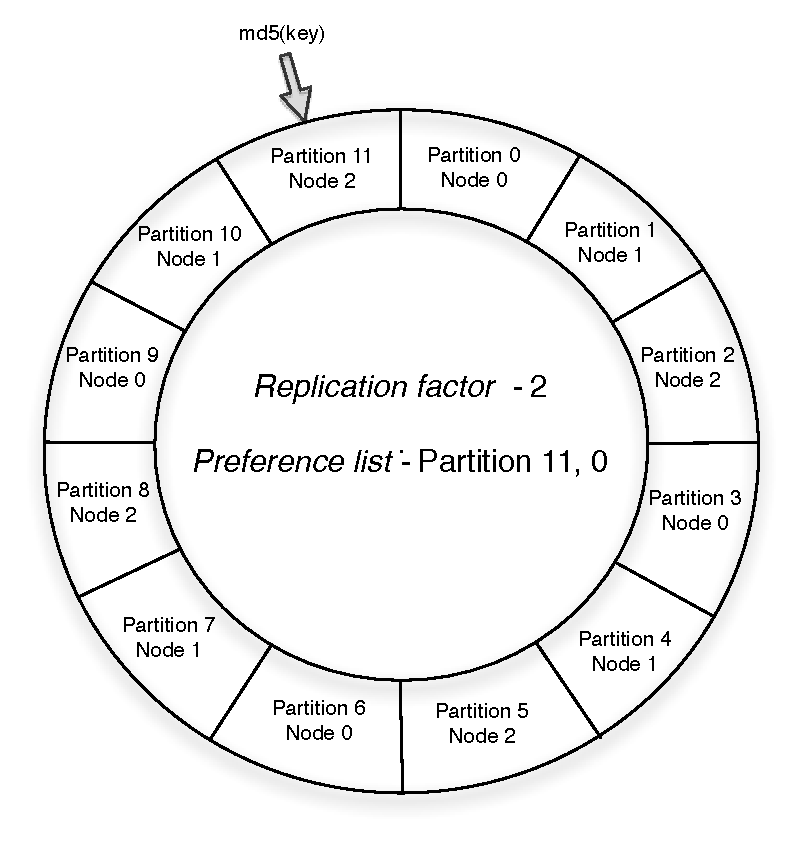
\includegraphics[scale=0.55]{images/hash.pdf}
  \caption{Hash ring with example preference list for (a) Dynamo's algorithm (b) Our zone based routing algorithm}
  \label{hash}
\end{figure}


The last module i.e. the storage layer implements the same $get$ and $put$ functions along with 2 other functions to support streaming operations (as shown in Figure \ref{storage_engines}). The ability to iterate over all tuples in a store is treated as a privileged command and has proved to be very helpful during debugging of data. 

\begin{figure}
\scriptsize
\begin{verbatim}
Iterator<K> keys() 
Iterator<Pair<K, VectorClock<V>>> entries()
\end{verbatim}  
\normalsize
\caption{Operations supported by all storage engines}
\label{storage_engines}
\end{figure}


Besides running the above stack, every node also runs a service which allow administrators to run restricted commands. Here we list some of the commands that we support.

\begin{itemize}
	\item \emph{Add / delete / truncate store} - Ability to add or delete a store without down time. We can also truncate the complete data without deleting the store. 
	\item \emph{Stream data} - We have the ability to stream data out of a store. If the store is read-write, we can stream data in as well. 
	\item \emph{Read-only store operations} - Trigger the batch fetch from Hadoop as well as other related operations. We will discuss this further in Section~\S\ref{sec:read_only}. 
	\item \emph{Slop operations} - Ability to manually trigger the periodic pushing job for hinted handoff. 
\end{itemize}

\begin{figure}
  \centering
    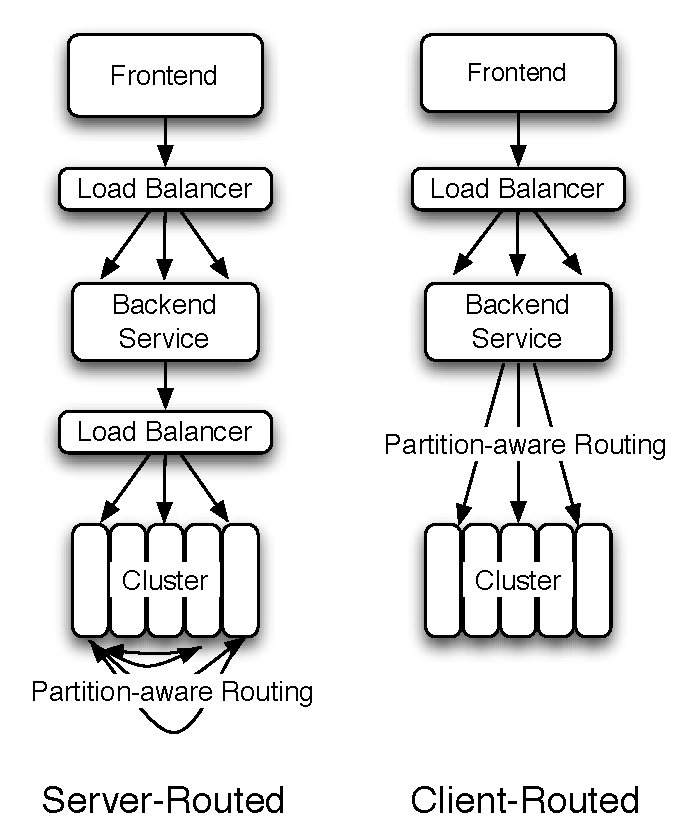
\includegraphics[scale=0.60]{images/fullstack.pdf}
  \caption{\projectname{} cluster usage in \linkedin{}}
  \label{fullstack}
\end{figure}


\noindent 
Now that we know the individual components, let us look at how \projectname{} is being used inside the complete \linkedin{} stack. As shown in Figure \ref{fullstack} we support both server side as well as client side routing. Client side routing requires an initial `bootstrap' step where-in it needs to retrieve two pieces of metadata - the cluster topology metadata and the store definitions. Since both of these are persisted on each and every \projectname{} node, the client initially hits a load balancer which in turn picks up a random live node to bootstrap from. Once the metadata has been retrieved the client gets the benefit of doing one less hop compared to server side routing since it knows exactly where the replicas for a key are. This is beneficial from a latency as well as throughput perspective since we have less number of services acting as bottlenecks. The disadvantage of the client side routing is that it makes the client side code-base large because of the extra routing and replication logic. Also, as we'll further explain in Section~\S\ref{sec:read_only:data_cycle:rebalancing}, it also makes rebalancing of data complicated since we now need a mechanism to change the cluster topology metadata on these live clients. 


% ========================== READ-ONLY-STORAGE ENGINE  ==========================================

\section{Read-only storage engine}
\label{sec:read_only}

Before we started writing our own custom storage engine we decided to
evaluate currently available storage engines, MySQL and Berkeley BD
(BDB), to see if they could fit our bulk loading use-case. Our
criteria for success was the ability to bulk load data as fast as
possible with minimum disk space overhead while still serving live
traffic.
 
We started by evaluating the various storage engines provided by
MySQL. The na\"ive approach of multiple insert statements is
problematic as every statement results in an incremental change to the
underlying index structure---in this case, a B$^{+}$ tree---which in
turn results in many disk seeks. To solve this problem, MySQL provides
a \sql{LOAD DATA} statement that tries to bulk update the underlying
index, but this requires a lock of the entire table if we the MyISAM
storage engine is used. InnoDB supports row-level locking, but comes
at the expense of substantial disk space overhead for every tuple.
Further, to achieve MyISAM-like performance with InnoDB, data must be
ordered by primary key.

We tried completely offloading the index construction to another
system as building the index on the serving system has isolation
problems, particularly with CPU and I/O. We attempted to build MyISAM
stores offline, opting to skip InnoDB due to the huge space
requirements. To do so, we leveraged the fact that MySQL allows
copying of database files from another node into a live database
directory; thereby automatically making it available for serving. We a
separate cluster where-in we would bulk load and then eventually copy
the data over to the live cluster, but this requires an extra
maintenance cost of a separate MySQL cluster with exactly the same
number of nodes as the live one. Further, the lack of ability to load
compressed data directly makes this process more time consuming, as
the data is copied multiple times between nodes: once as a flat file
to the bulk load cluster, then the internal copy during the LOAD
statement, and finally the raw data copy to the actual live database. 

The previous solution is not ideal due to its dependency on the
redundant MySQL servers, which makes the complete process prone to
failure downtimes. Instead, what if we could use the inherent fault
tolerance and parallelism of Hadoop and build individual node /
partition level data stores which could be pulled over by
\projectname{} for serving? The large-scale adoption of HDFS as the
data sink makes it an ideal location to act as our source of data:
most data is ETL'd into HDFS for storage and later processing anyway.
So the next attempted approach was to use Hadoop and a good single
node node high performance storage engine to generate smaller data
stores in parallel. That is, a Hadoop job reads data from a source in
HDFS, re-partitions on a per node basis, and finally writes the data
to individual stores (for example, BDB) on the local filesystem in the
reducer phase. The number of reducers were equal to the number of
nodes, but could have easily been further split on a per partition
basis. This data is then read from the local filesystem and copied
onto HDFS from where it can be read by \projectname{}. The benefits of
this approach is that it leverages Hadoop's fault tolerance to build
the indexes offline, but it suffers from an extra copy from the local
file system the reducer nodes to HDFS---which can become a real
bottleneck with terabytes of data. 

From the above experiments we came to the conclusion that we required
our own custom storage engine. Our new custom storage engine, along
with its complete pipeline, should have the following properties. 
\begin{compactitem}
\item \emph{No performance impact on live requests}. The incoming
requests to the live store must not be impacted during the data load.
There is a tradeoff between modifying the current index on the live
server and finishing the bulk load as fast as possible, but that can
increase I/O and hurt performance. As a result, we completely rebuild
the index offline. 
\item \emph{Fault tolerance and scalability}. Every step of the data
load pipeline should be able to handle failures. Hadoop, but its
ability to deal with failures, is used as the computation layer for
building the index. Similarly, HDFS's replication provides
availability. Finally \projectname{} is used as the serving layer, as
its routing strategies provide replica fall back in the case of
failures. All of these systems can easily scale horizontally due to
their already existing support for expansion without downtime. 
\item \emph{Rollback}. The general trend we notice in our business
that data is treated more like code: incorrect or incomplete data
could have been due to algorithm changes or source data problems. To
minimize the time in error, the storage engine must support very fast
rollback to the previous dataset.
\end{compactitem}

Our new data deployment pipeline consists of a new storage engine that
is built in Hadoop (\S\ref{sec:read_only:storage_format}), versioned
for rollback (\S\ref{sec:read_only:versioning}), and deployed. We
finally conclude by explaining how it fits into the complete data
deployment cycle along with some real world production scenarios and
how we dealt with it. 

% ========================== READ-ONLY-STORAGE ENGINE  - STORAGE FORMAT ==========================================

\subsection{Storage format}
\label{sec:read_only:storage_format}

Many storage formats try to build data structures that keep the data
memory-resident in the process address space, ignoring the effects of
the operating system's page cache. A classical example is the InnoDB
storage engine of MySQL, which buffers both key and data pages
resulting in double caching at both OS as well as MySQL level. The
several orders of magnitude latency gap between the page cache and
disk means the only real performance benefit by maintaining our own
structure is for elements already in the page cache. In fact, this
custom structure may even start taking memory away from the page
cache. Rather, this motivated the need of our storage engine to
exploit the page cache instead of maintaining our own complex data
structure. Since our data is immutable, \projectname{} memory maps the
entire index into the address space. Further, since \projectname{} has
been written in Java and runs on the JVM, delegating the memory
management to the operating system eases garbage collection tuning.

\begin{figure}
  \centering
    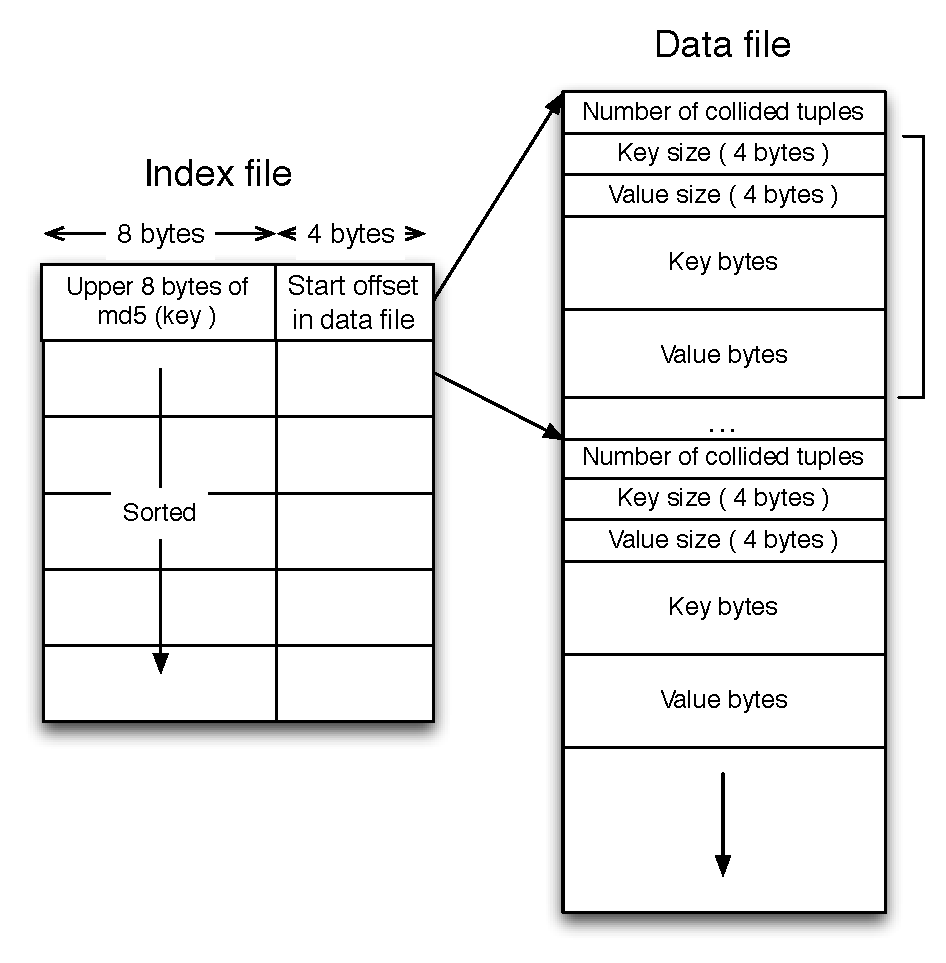
\includegraphics[scale=0.45]{images/storage_format.pdf}
  \caption{Chunk file format}
  \label{storage_format}
\end{figure}

Figure~\ref{storage_format} shows the structure of the storage
engine's data and index files. 

The data is split into multiple chunks where every chunk is a pair of
data and index files. This split is necessary to achieve parallelism
for store building in Hadoop. The system builds multiple chunks for
every partition-replica bucket. We have set a standard naming
convention for all our chunk files. It follows the pattern
\verb=<partition id>_<replica id>_<chunk id>.= \verb=<data or index>=,
where \verb=partition id= is the id of the primary partition and
\verb=replica id= is a number between 0 to `replication factor'-1.
Once a key hashes to a particular node, we classify it into the
correct \verb=partition id= + \verb=replica id= bucket. For example
the key in Figure \ref{hash}, present in a store using consistent
hashing, would fall into the buckets 11\_0 (on node 2) and 11\_1 (on
node 0). 

The system takes all the tuples in this bucket, splitting them further
into multiple smaller chunks. The table \ref{tab:node_to_chunk} below
shows the various bucket names (where every bucket will contain
multiple chunks and each chunk will in turn contain an index and data
file) for a store with consistent hash routing and replication factor
2. This assumes that the cluster has the same partition ring topology
as shown in Figure \ref{hash}. Our initial design started with the
simpler scheme of one bucket per node (i.e. multiple chunks stored on
a node with no knowledge about partitions), but this smaller
granularity is necessary to aid in
rebalancing~(\S~\ref{sec:read_only:data_cycle:rebalancing}).

\begin{table}
\begin{center}
    \begin{tabular}{ | c | c | }
    \hline
    Node Id & Chunk files \\ \hline
    0 &  0\_0, 3\_0, 6\_0, 9\_0,      2\_1, 5\_1, 8\_1, 11\_1	\\
   1 &   1\_0, 4\_0, 7\_0, 10\_0,      0\_1, 3\_1, 6\_1, 9\_1		\\
   2 &    2\_0, 5\_0, 8\_0, 11\_0,    1\_1, 4\_1, 7\_1, 10\_1		\\
\hline
    \end{tabular}
\end{center}
 	\caption{Node to chunk mapping}
 	\label{tab:node_to_chunk}
\end{table}

The index file is a compact structure containing the sorted upper
8~bytes of the MD5 of the key followed by the 4~byte offset of the
corresponding value in the data file. This simple sorted structure
allows us to easily leverage Hadoop, where mappers and reducers do not
have much memory. Further, preliminary tests also showed that the
index files were generally order of magnitude smaller than the data
files and hence, could safely fit into the page cache.

An interesting optimization is that the full 16 bytes of the MD5 of
the key is not necessary. We had initially started by using the full
MD5 signature, but over time we noticed multi-tenant performance
problems: stores were stamping on each others pages in the page cache.
To alleviate this problem, we needed to cut down on the amount of data
being memory mapped, which can be achieved by reducing the available
key-space and accepting collisions in the data file. 

Our optimization proceeded as follows and can be mapped to the classic
birthday paradox: if we want to retrieve $n$ random integers from a
uniform distribution of range $[1, x]$, the probability that at least
2 numbers are the same is:
\begin{equation}
1 - e^{\frac{-n(n-1)}{2x}}
\end{equation}
Mapping this to our scenario, $n$ is generally our 120 million member
user base, while the initial value of $x$ is $2^{128} - 1$ (16 bytes
of MD5). The probability of collision in this scenario was close to 0.
A key-space of 4 bytes (i.e. 32 bits) yields an extremely high
collision probability of:
\begin{equation}
1 - e^{\frac{(-120*10^{6} * (120*10^{6} - 1)}{2 * (2^{32} - 1)}} \sim 1
\end{equation}
Instead, a compromise of 8 bytes (i.e. 64 bits) produces:
\begin{equation} 
1 - e^{\frac{(-120*10^{6} * (120*10^{6} - 1)} { 2 * (2^{64} - 1 )}} < 0.0004
\end{equation}
The probability of more than one collision is even smaller. Thus, by
decreasing the number of bytes of the MD5 of the key we were able to
cut down the index size by 40\%, thereby making our clusters more
multi-tenant. The size of the keys-space is an optional parameter the
admin may set depending on the semantics of the data. Unfortunately,
this came at the expense of us having to save the keys in the data
file to use for lookups and handle the rare collisions in the data
files.

The data file is similarly a very highly packed structure where we
store the number of collided tuples followed by a set of collided
\verb=[key size, value size, key, value]= list. The important thing to
remember here is that we store the raw key bytes instead of the MD5-ed
key bytes in order to do a comparison during reads. 

% ========================== READ-ONLY-STORAGE ENGINE  - VERSIONING ==========================================

\subsection{Versioning of data}
\label{sec:read_only:versioning}

One of our requirements was the ability to rollback the data. The
above chunk files need to be stored in a layered format so as to allow
rollback. Every time a new copy of the complete data-set is created,
the system needs to demote the previous copy to an older state.
Following is how the data is structured for the read-only stores on a
\projectname{} node. 

Every store is represented by a directory which then contains various
``versions'' of the data. Since the data in all the version
directories, except the serving one, are inactive we are not affecting
the page cache usage and hence the latency. Since disk is cheap and
rollbacks are important, keeping some previous copies of the data
(configurable by the user or admin) is beneficial.

Deploying a new data version is as simple as starting a new version
folder and changing the symbolic link to the latest data. A rollback
is as simple as changing the symbolic link to a previous version
folder and swapping the data in. 

% ========================== READ-ONLY-STORAGE ENGINE  - CHUNK GENERATION ==========================================

\subsubsection{Chunk generation}
\label{sec:read_only:chunk_generation}

Construction of the chunk files for all \projectname{} nodes is a
single MapReduce job; the pseudo-code representation is shown in
Figure~\ref{fig:mapreduce-chunk-generation}.

\begin{figure}
\centering

\scriptsize
\begin{verbatimtab}
# numChunks - Number of chunks per bucket
# repFactor - Replication factor of store
# topBytes(array, N) - Read top N bytes from array

# K - raw key
# V - raw value
map(K, V):
  K' = makeKey(K, V)     	# Create Spock key
  V' = makeValue(K, V)   	# Create Spock value
  MD5K' = md5(K')
  [partitionIds] = preferenceList(MD5K')
  replicaId = 0			# Replica type - Primary (0)
  foreach ( partitionId in partitionIds )
    nodeId = partitionToNode(partitionId)
    emit(topBytes(MD5K', 8),<nodeId, partitionId, replicaId, K',V'>) 
    replicaId++     

# K - Top 8 bytes of MD5 of Spock key
# V - <Node Id,Partition Id,Replica Id,Spock key,Spock value>
# return reducer id
partitioner(K, V) : int
  chunkId = topBytes(K, size(int)) % numChunks
  return ((V.partitionId*repFactor+replicaId)*numChunks)+chunkId
 
# K - Same as partitioner
# V - Same as partitioner
# position - Offset in data file. Start with 0
reduce (K, Iterator<V> iter)
  writeIndexFile(K)
  writeIndexFile(position)
  writeDataFile(iter.size)   # number of collided tuples
  foreach ( V in iter )
    writeDataFile(V.K'.size) # int
    writeDataFile(V.V'.size) # int
    writeDataFile(V.K')
    writeDataFile(V.V')
    position += (2 * size(int) + V.K'.size + V.V'.size)
\end{verbatimtab}
\caption{MapReduce for Chunk generation}
\label{fig:mapreduce-chunk-generation}
\end{figure}

The Hadoop job consists on a simple map phase which partitions the
data depending on the routing strategy where the partitioner redirects
keys to the correct reducer; the reduce phase writes the data to a
single chunk (i.e. a data and index file). Due to Hadoop's generic
\term{InputFormat} mechanics, any source data can be converted to
\projectname{}. This phase then emits the upper 8~bytes of MD5 of the
\projectname{} key $N$~times as the map phase key with the map phase
value equal to a grouped tuple of node id, partition id, replica id
and the raw \projectname{} key and value. The custom partitioner then
generates the chunk id from this key. Since there is a fixed number of
chunks on a per partition-replica basis, the chunk id is generated
with a simple mod of the number of chunks. The partitioner uses the
partition id, replication factor of the store and the chunk id to
route the key to the correct reducer. Finally, every reducer is
responsible for a single chunk, meaning that by having more chunks,
once can increase the parallelism during the build phase. Since Hadoop
automatically sorts the data based on the key, the process receives
data in the order necessary for the output data files and can simply
append to index and data file on HDFS with no extra processing
required.  

% ========================== READ-ONLY-STORAGE ENGINE  - SEARCH ==========================================

\subsubsection{Search}
\label{sec:read_only:search}

To find a key, the system needs to run the current routing strategy to
determine which partitions (and so nodes) will need to query for the
key. The following is a sketch of the algorithm to find the data. 

\begin{enumerate}
  \item Calculate the MD5 of the key
  \item Generate partition id, replica id (which replica were we
searching for when we came to this node?) and chunk id (By taking the
first 4 bytes of the MD5-ed key, modulo the number of chunks)
  \item Go to the store's folder and find the chunk files having the
above chunk id in the bucket (partition id and replica id). 
  \item Do a binary search using the top 8~bytes of
the MD5-ed key as the search key in the index file. This is easy to do
since we have fixed space requirements for every key (12 bytes - 8
bytes for key and 4 bytes for offset) thereby not requiring any
internal pointers within the index file. For example to find the data
location of the $i$th element in the sorted index is a simple jump to
the offset 12 * $i$ + 8 from where we can read the offset to the data
file.  
  \item Once we have the offset in the data file we iterate over all
the collided tuples in the data file, comparing the keys. If we find
the key we are looking for, we return the corresponding value.
\end{enumerate}

The most time consuming step above is the search in the index file. A simple binary search in an index of size 1 million keys can result in around 20 key comparisons. This means if the cache is completely not cached we will be doing 20 expensive disk seeks just to read one value. To partially solve this problem while fetching the files from HDFS we transfer the index files after all data files. This helps a little since now the index files might still be in the operating system's page cache thereby helping decreasing the number of times we hit the disk. Unfortunately this small optimization still doesn't help in the scenario when we do a rollback of data to a previous version folder. 

A lot of previous work has been done in the area of search algorithms for disk files which are sorted. One of these algorithms includes Interpolation search\cite{manolopoulos}. This search strategy is a little smarter than binary search, in that instead of always looking into the middle of the search range in the array, it uses the key distribution to predict the approximate location of the key. This works very well for uniformly distributed keys and drops the search complexity from O(log N) to O (log log N). This definitely helps in the completely un-cached scenario since we are dropping the number of key lookups. Saving every key comparison in the un-cached scenario is beneficial since every lookup costs a couple of milliseconds. The one disadvantage of interpolation search is that the rate of data now becoming cached decreases due to less areas of the index that we are accessing. 

Other than the above algorithms, we also looked into other strategies like Fast and Pegasus. As proved in \cite{manolopoulos}, most of these are better suited for non-uniform distributions. Since we can assume that MD5 provides a good uniform distribution the speed-up involved in using these other algorithms is very small. 

% ========================== READ-ONLY-STORAGE ENGINE  - COMPLETE DATA CYCLE ==========================================

\subsection{Complete data cycle}
\label{sec:read_only:data_cycle}

Figure \ref{cycle} shows the complete data cycle that eventually results in new data being swapped into a \projectname{} store. 

\begin{figure}
  \centering
    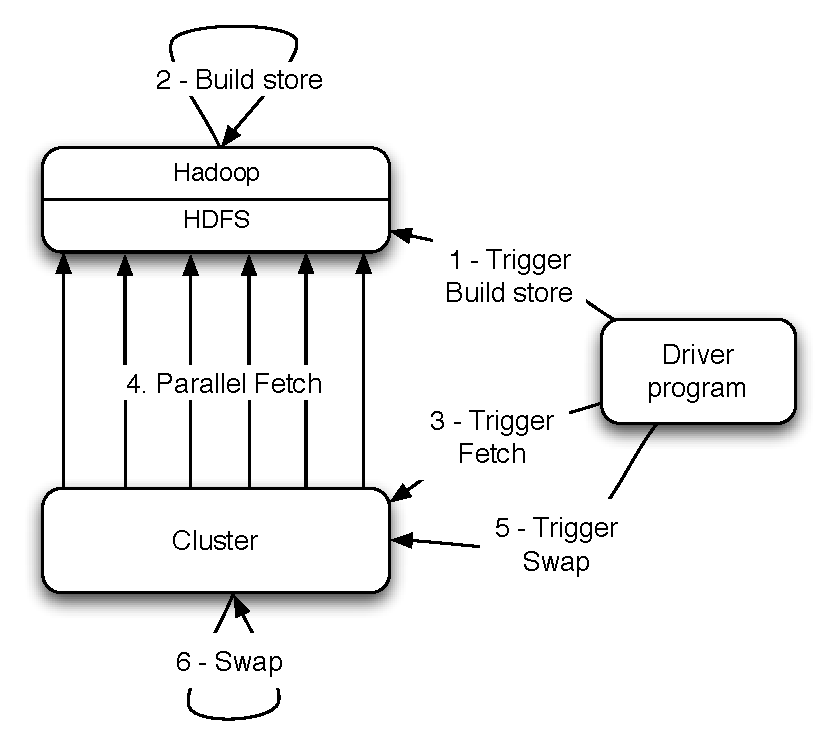
\includegraphics[scale=0.60]{images/cycle.pdf}
  \caption{Read-only data cycle}
  \label{cycle}
\end{figure}

The initiator of this complete fetching and swapping of new data process can be either Azkaban or a standalone driver program. Azkaban\cite{azkaban} is a simple batch scheduler built at \linkedin{} which allows you to schedule Hadoop as well other offline batch jobs. Individual end products schedule batch Hadoop and Pig jobs to run algorithms on the raw data which finally loads the data to \projectname{} as the last step. The last step starts by Azkaban triggering our Hadoop job described in Section~\S\ref{sec:read_only:chunk_generation}. This job generates the data on a per node basis and stores it into HDFS. While streaming the data out onto HDFS we also calculate the checksum on a per node basis. This checksum is calculated by running an MD5 on the individual MD5s of all the chunk files in a node directory. This checksum value is then stored in a special file $.metadata$ in every node folder. 

Once the Hadoop job is complete Azkaban triggers a fetch request on all \projectname{} nodes along with information about the root directory path on HDFS. This request is received by our `administrative service' on every node which then initiates an HDFS client and starts a parallel fetch for the node folder it is responsible for. This data is stored into a new version directory whose version number could either be specified as a parameter by Azkaban or defaulted to (previous version number + 1). While the data is being fetched from HDFS we also calculate the same checksum so as to cross-check it with the stored checksum in the $.metadata$ file. While building this fetch layer we made sure to keep the interface generic so as to support fetching data from non-HDFS locations as well. The other important decision we made here was to adopt the pull model instead of the push model. This allows the \projectname{} node to now throttle the fetches in case of any latency problems. 

The next step after the fetch is complete is to swap the new data-set in and swap the older version out. For Azkaban to know when to initiate a swap it needs to know when the fetch has successfully completed. Since the fetch process can take a long time we provide a hook in the administrative service for Azkaban / standalone program to keep checking so as to get a progress report of how much we have finished fetching. Finally after the fetch is complete Azkaban triggers a swap operation on all nodes. This operation is co-ordinated using a read-write lock in our storage engine. We obtain a write lock when the swap starts during which we do the following - close all open file in the current version directory, change the symbolic link to the new version directory and finally open all chunk files and memory map the indexes. This complete operation doesn't take more than a few milliseconds since it is not dependent on the file size information. To provide global atomic semantics we make sure that all the nodes have successfully swapped their data. If any of the swaps have failed, we run an extra step to rollback the data on the successful nodes.


% ========================== READ-ONLY-STORAGE ENGINE  - COMPLETE DATA CYCLE - SCHEMA CHANGE ==========================================

\subsubsection{Schema upgrades}
\label{sec:read_only:data_cycle:schema_upgrades}

As engineers iterate on their products there are bound to be changes in the underlying data format of the values that they want to expose to the user. Common example of this is if a product wants to add a new dimension to their value. For the same \projectname{} supports the ability to change the schema of the key and value without any downtime. Since read-only data is static and we can do a complete load of the full data-set every time we can easily change the schema during one of our loads. But for the client to transparently handle this change we need to added a special byte in our most used serialization format, Binary JSON, to encode the version of the schema. This same version information is saved in the stores metadata which the clients pick up during bootstrapping. The clients then maintain a mapping from version id to corresponding schema. So if a data fetch takes place with the new schema, during the read we toggle to the right version id and pick up the corresponding schema. Similarly if a rollback of data takes place the client will toggle back to an older version of schema and be able to parse the data with no downtime. 

% ========================== READ-ONLY-STORAGE ENGINE  - COMPLETE DATA CYCLE - REBALANCING ==========================================

\subsubsection{Rebalancing}
\label{sec:read_only:data_cycle:rebalancing}

Rebalancing is a major feature which allows \projectname{} to easily add or rebalance data around on a live cluster without down time. This feature was initially written for the read-write stores but easily fits into the read-only cycle due to the static nature of the data. Our smallest unit of rebalancing is a partition. In other words addition of a new node translates to giving the ownership of some partitions to it. The rebalancing process is run by a rebalancing tool which co-ordinates the full process. The following are the steps that are followed during the addition of a new node. 

\begin{itemize}
	\item Provide the rebalancing tool with the future cluster topology metadata.
	\item Using the future cluster topology metadata, generate list of all primary partitions that need to be moved
	\item Do the following steps for every `batch' of primary partitions. The reason behind moving the partition in small batches is that it makes the process checkpoint-able without having to re-fetch too much data. 
		\begin{itemize}
			\item Generate intermediate cluster topology metadata which is current cluster topology with changes in ownership of `batch' of partitions moved
			\item Use intermediate cluster topology metadata to generate a set of steps that need to be run to finish rebalancing. In this process we also need to take care of all the secondary replica movements that might be required due to the primary partition movement. This plan is a set of donating node id and stealing node id pairs along with the chunk files being moved. 
			\item Initiate asynchronous processes (through the administrative service) on all the stealer nodes which then start stealing chunk files from their corresponding donor nodes. The data is copied into the same version directory which is currently serving live traffic. We also make these nodes to go into a `rebalancing state' thereby not allowing any new fetches and swaps from taking place. 
			
			Here it is important to note that the granularity of the bucket we selected made this process as simple as just a copy of files. If we had defined a bucket to be on a per node basis i.e. have multiple chunks on a per node basis, we would have had to iterate over all the keys on the node and find the correct key set belonging to the moving partition. Further we would then need to merge this key set with the live serving index on the stealer node's end. 
			\item Once the fetches have completed the rebalancing tool updates the intermediate cluster topology on all the nodes while also doing an atomic swap of data on the stealer and donor nodes. 
			
			This topology change information also needs to be propagated to all the upper services using client side routing. We propagate this information as a lazy process where-in the clients still use the old metadata. If they contact a node with a request for a key in a partition which the node is no more responsible the node sends a special exception. This special exception then results in a re-bootstrap step along with a retry of the previous request.
		\end{itemize}
\end{itemize}

The rebalancing tool has also been designed to handle failure scenarios elegantly. Failure during a fetch is not a problem since we haven't swapped the data in. But failure during the swap requires us to rollback the cluster topology to the last good cluster topology while also rolling back the data on the successful nodes. Let us end this section by demonstrating a simple example showing the plan generation. We will run this for the same hash ring shown in Figure \ref{hash} with a store using consistent hashing. We introduce a new node (Node 3) to whom we will initially pass the responsibility of partitions 3. Table \ref{tab:new_node_to_chunk} shows the new chunk mapping, while Table \ref{tab:rebalance_plan} shows the simple plan that would be generated as a part of rebalancing. 

\begin{table}
\begin{center}
    \begin{tabular}{ | c | c | }
    \hline
    Node Id & Chunk files \\ \hline
    0 &  	0\_0, 6\_0, 9\_0,      			5\_1, 8\_1, 11\_1 			\\
   	1 &   	1\_0, 4\_0, 7\_0, 10\_0,      	0\_1, 3\_1, 6\_1,9\_1  		\\
   	2 &    	2\_0, 5\_0, 8\_0, 11\_0,    	1\_1, 4\_1, 7\_1, 10\_1		\\
   	3 &   	3\_0,                         	2\_1 						\\
\hline
    \end{tabular}
\end{center}
 	\caption{New node to chunk mapping}
 	\label{tab:new_node_to_chunk}
\end{table}

\begin{table}
\begin{center}
    \begin{tabular}{ | c | c | c | }
    \hline
    Stealer Node Id & Donor Node Id & Chunks to steal \\ \hline
    3 &  0 & 3\_0, 2\_1	\\
\hline
    \end{tabular}
\end{center}
\caption{Rebalancing plan generated}
\label{tab:rebalance_plan}
\end{table}




